\documentclass[UTF8]{ctexart}
\usepackage{ctex} 
\usepackage{tikz}
\usepackage{graphicx}
\usepackage{amsmath}  
\usepackage{float}
\usepackage{geometry}   
\usepackage{setspace}  
\usepackage{esint}  
\graphicspath{{doc_img/}}
\title{五子棋}
\author{靓仔语塞。jpg\\
林天皓 \ 龙行健 \ 陈逸铭 \ 廖洋 \ 高远 \ 艾刚正}
\date{\today}
\begin{document}
\maketitle
\newpage
\tableofcontents
\newpage
\section{简介}
本程序实现了五子棋人人对战,人机对战的功能,支持悔棋,切换皮肤,回合数显示,记录走棋过程,棋局复盘等功能。\\
\paragraph{}
主界面如下:
\begin{figure}[H]
    \centering
    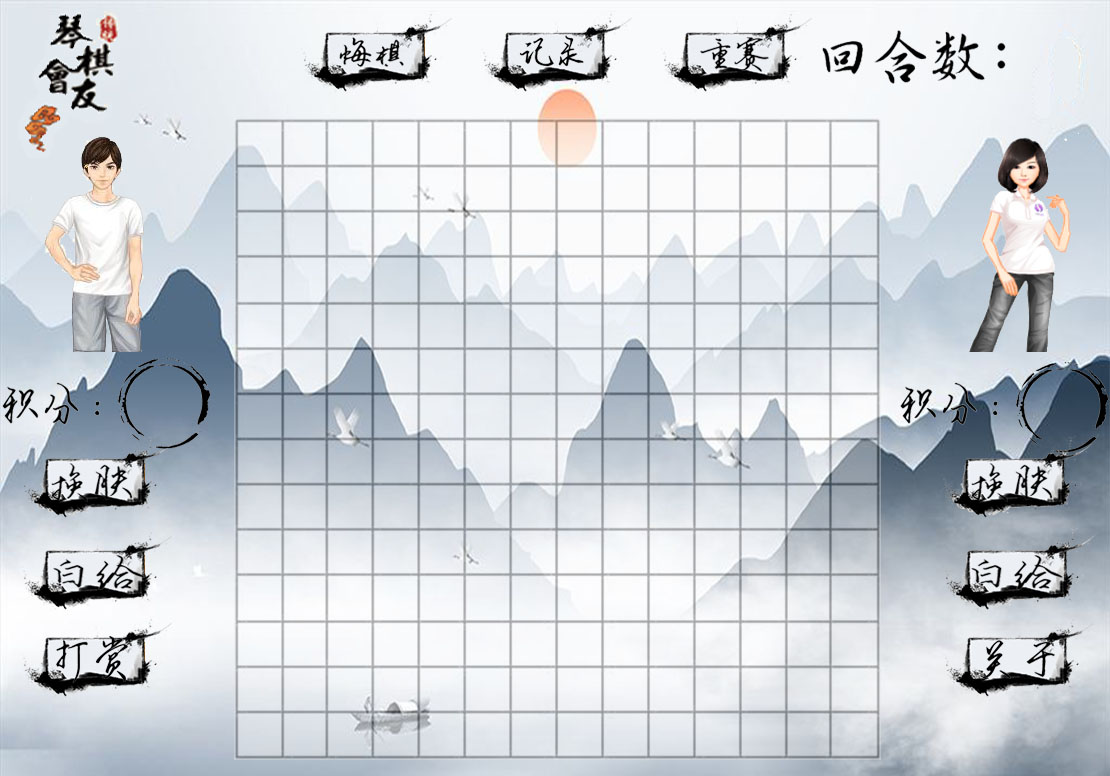
\includegraphics[scale=0.4]{qipan.jpg}
    \caption{棋盘}
\end{figure}
\section{程序架构}
\begin{figure}[H]
    \centering
    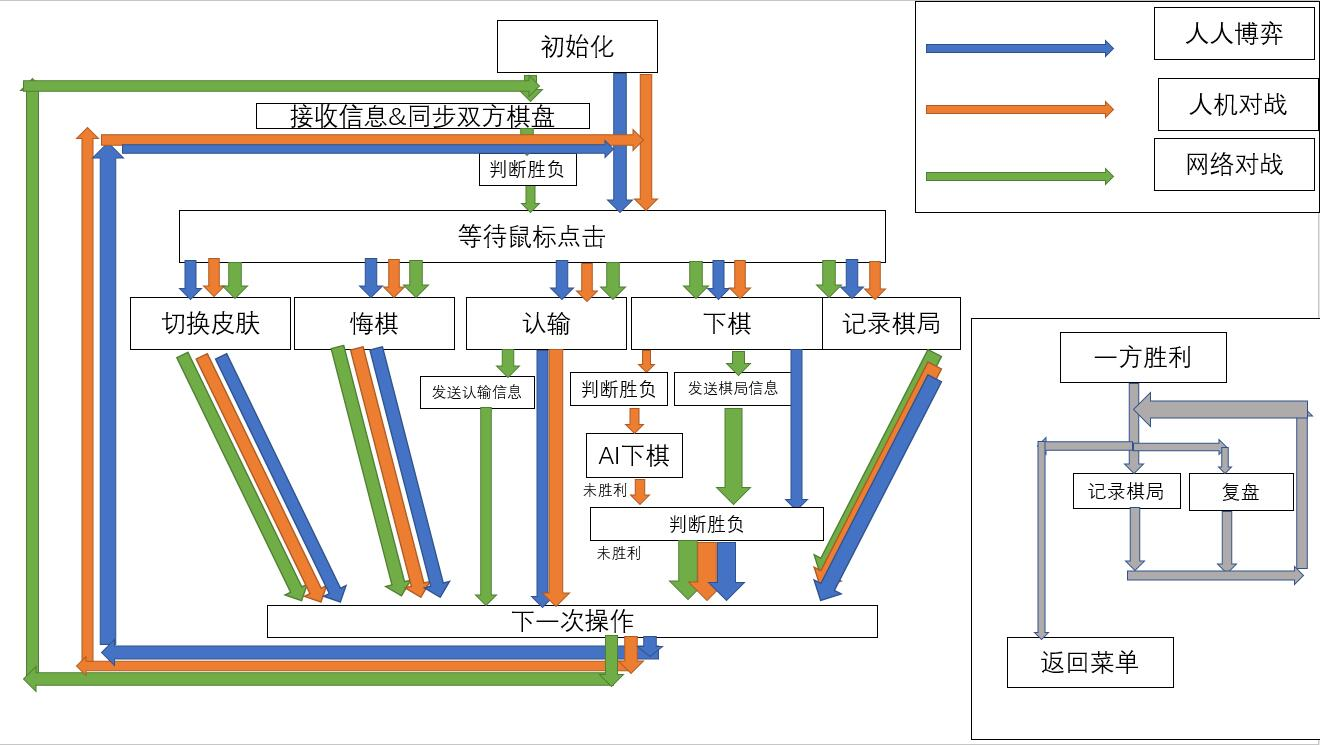
\includegraphics[scale=0.48]{liuchengtu.jpg}
    \caption{整体架构流程}
\end{figure}
\section{程序函数介绍}
\subsection{主函数}
\begin{figure}[H]
    \centering
    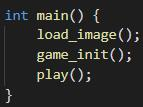
\includegraphics[scale=2.0]{1.jpg}
    \caption{2}
\end{figure}
\subsection{载入图片}
\begin{figure}[H]
    \centering
    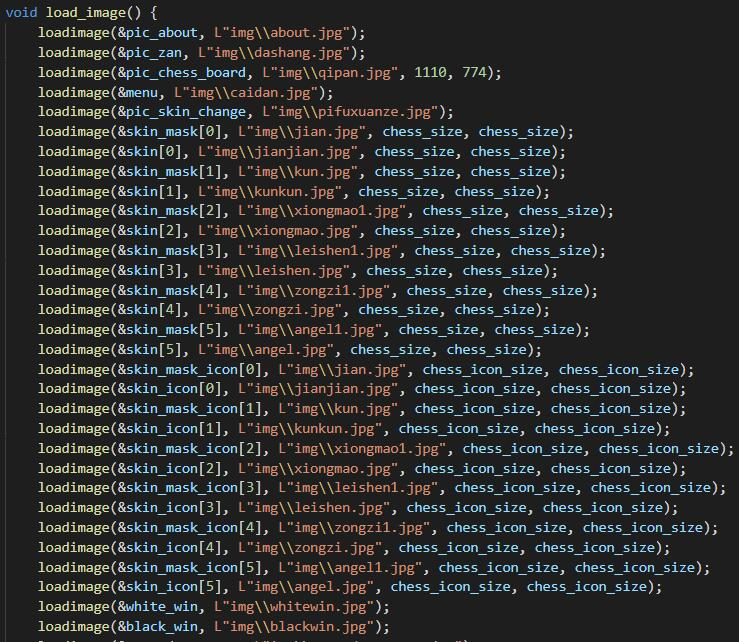
\includegraphics[scale=0.8]{2.jpg}
\caption{3}
\end{figure}
\subsection{鼠标按钮判断}
\begin{figure}[H]
    \centering
    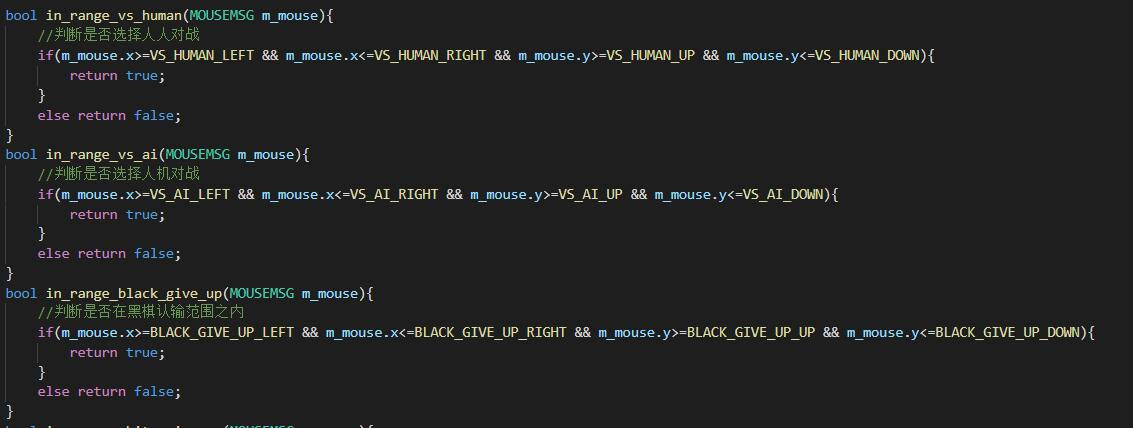
\includegraphics[scale=0.6]{3.jpg}
\caption{4}
\end{figure}
\subsection{初始化}
\begin{figure}[H]
    \centering
    
\includegraphics[scale=1.0]{4.jpg}
\caption{5}
\end{figure}
\subsection{选择人人对战或者人机对战}
\begin{figure}[H]
    \centering
    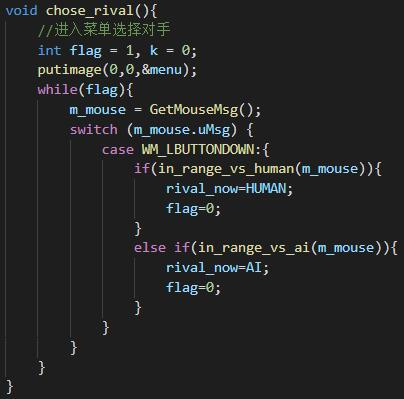
\includegraphics[scale=1.0]{5.jpg}
\caption{6}
\end{figure}
\subsection{游戏中内容}
\begin{figure}[H]
    \centering
    
\includegraphics[scale=1.0]{6.jpg}
\caption{7}
\end{figure}
\subsection{下棋}
\begin{figure}[H]
    \centering
    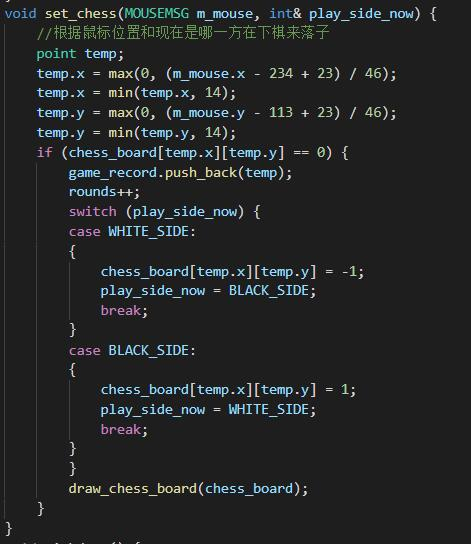
\includegraphics[scale=1.0]{7.jpg}
\caption{8}
\end{figure}
\subsection{悔棋}
\begin{figure}[H]
    \centering
    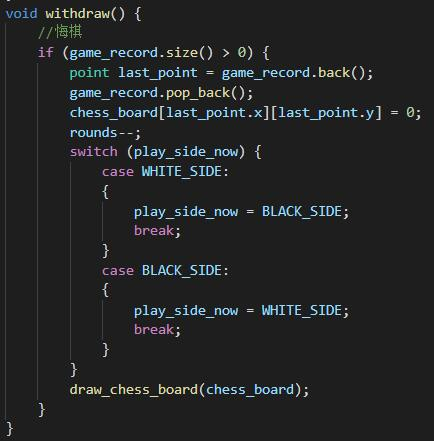
\includegraphics[scale=1.0]{8.jpg}
\caption{9}
\end{figure}
\subsection{暂停,按鼠标左键继续}
\begin{figure}[H]
    \centering
    
\includegraphics[scale=1.0]{9.jpg}
\caption{10}
\end{figure}
\subsection{画棋盘}
\begin{figure}[H]
    \centering
    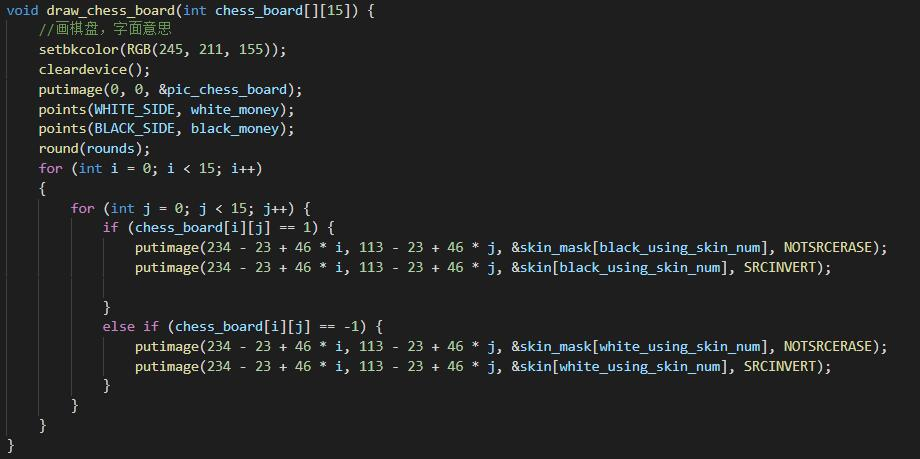
\includegraphics[scale=0.65]{10.jpg}
\caption{11}
\end{figure}
\subsection{判断是否五连}
\begin{figure}[H]
    \centering
    
\includegraphics[scale=0.60]{11.jpg}
\caption{12}
\end{figure}
\subsection{是否有一方胜利}
\begin{figure}[H]
    \centering
    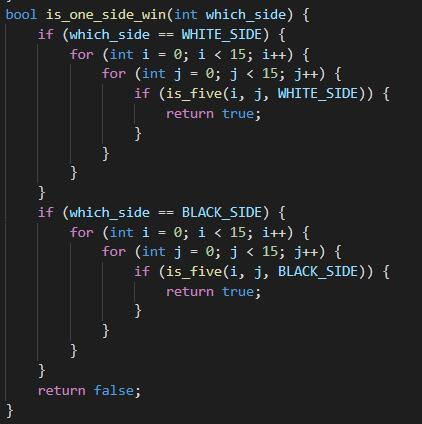
\includegraphics[scale=0.7]{12.jpg}
\caption{13}
\end{figure}
\subsection{重来}
\begin{figure}[H]
    \centering
    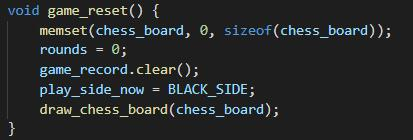
\includegraphics[scale=1.0]{13.jpg}
\caption{14}
\end{figure}
\subsection{复盘}
\begin{figure}[H]
    \centering
    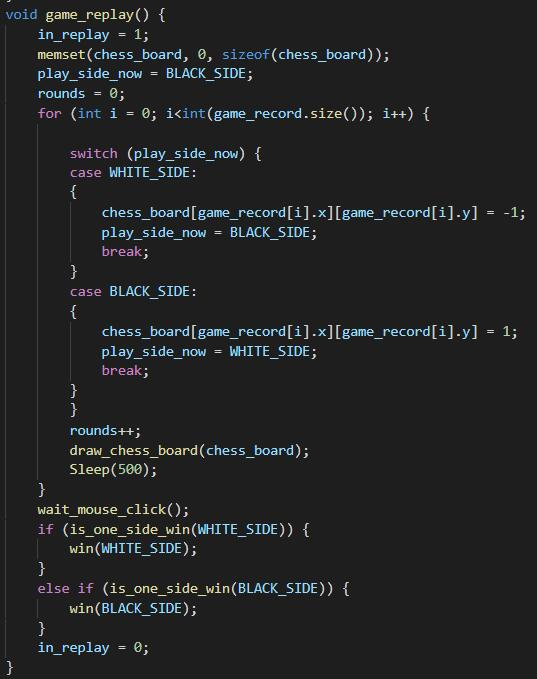
\includegraphics[scale=1.0]{14.jpg}
\caption{15}
\end{figure}
\subsection{胜利后的画面}
\begin{figure}[H]
    \centering
    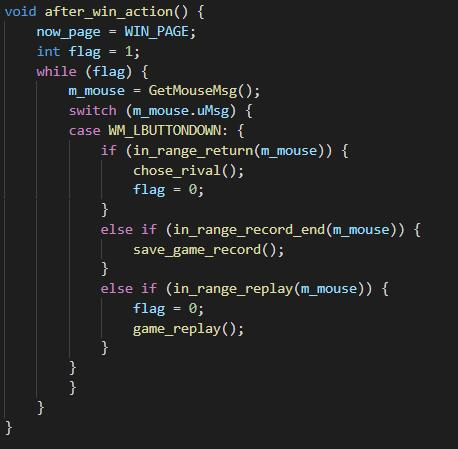
\includegraphics[scale=1.0]{15.jpg}
\caption{16}
\end{figure}
\subsection{画积分数}
\begin{figure}[H]
    \centering
    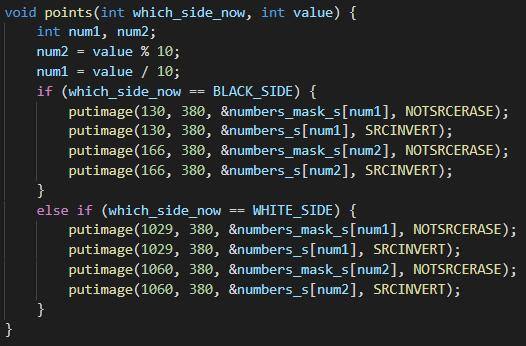
\includegraphics[scale=1.0]{16.jpg}
\caption{17}
\end{figure}
\subsection{画回合数}
\begin{figure}[H]
    \centering
    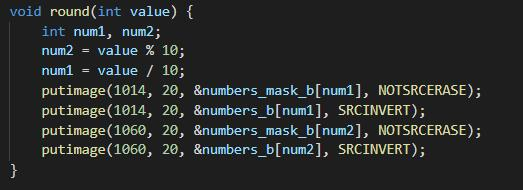
\includegraphics[scale=1.0]{17.jpg}
\caption{18}
\end{figure}
\subsection{一方胜利后的动作}
\begin{figure}[H]
    \centering
    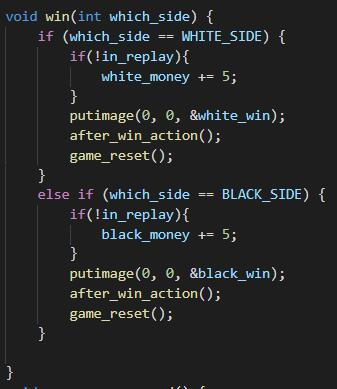
\includegraphics[scale=1.0]{18.jpg}
\caption{19}
\end{figure}
\subsection{保存下棋记录}
\begin{figure}[H]
    \centering
    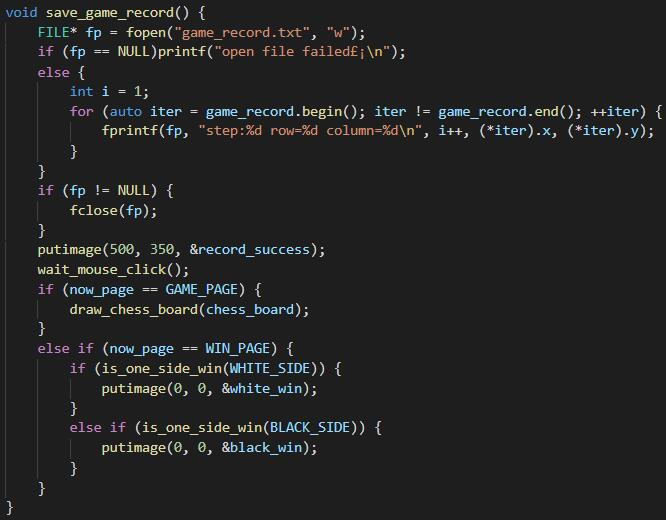
\includegraphics[scale=0.9]{19.jpg}
\caption{20}
\end{figure}
\subsection{展示皮肤}
\begin{figure}[H]
    \centering
    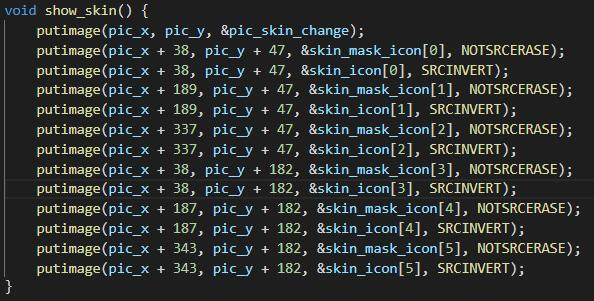
\includegraphics[scale=0.8]{20.jpg}
\caption{21}
\end{figure}
\subsection{选择皮肤}
\begin{figure}[H]
    \centering
    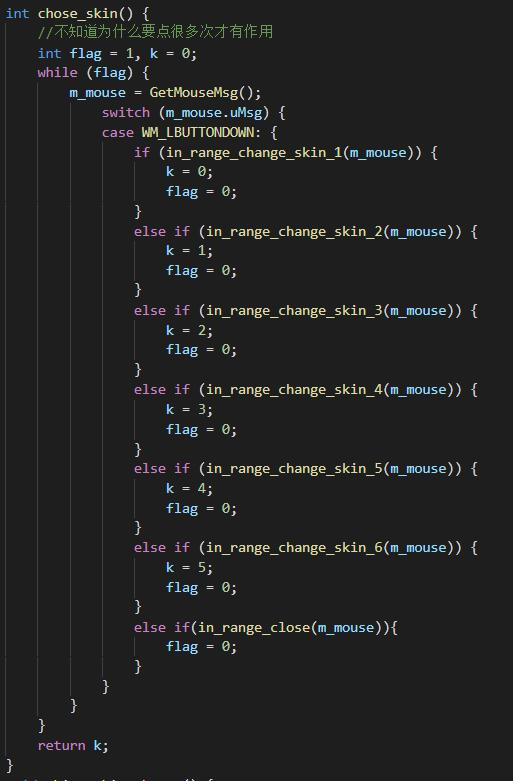
\includegraphics[scale=1.0]{21.jpg}
\caption{22}
\end{figure}
\subsection{白色方换皮肤}
\begin{figure}[H]
    \centering
    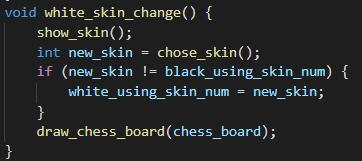
\includegraphics[scale=1.0]{22.jpg}
\caption{23}
\end{figure}
\subsection{黑色方换皮肤}
\begin{figure}[H]
    \centering
    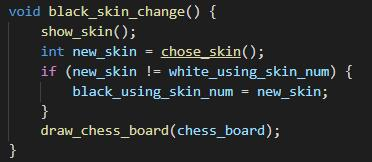
\includegraphics[scale=1.0]{23.jpg}
\caption{24}
\end{figure}
\subsection{判断两头周围是否有棋子}
\begin{figure}[H]
    \centering
    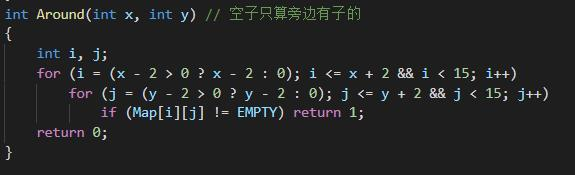
\includegraphics[scale=1.0]{24.jpg}
\caption{25}
\end{figure}
\subsection{输入几联,输出得分}
\begin{figure}[H]
    \centering
    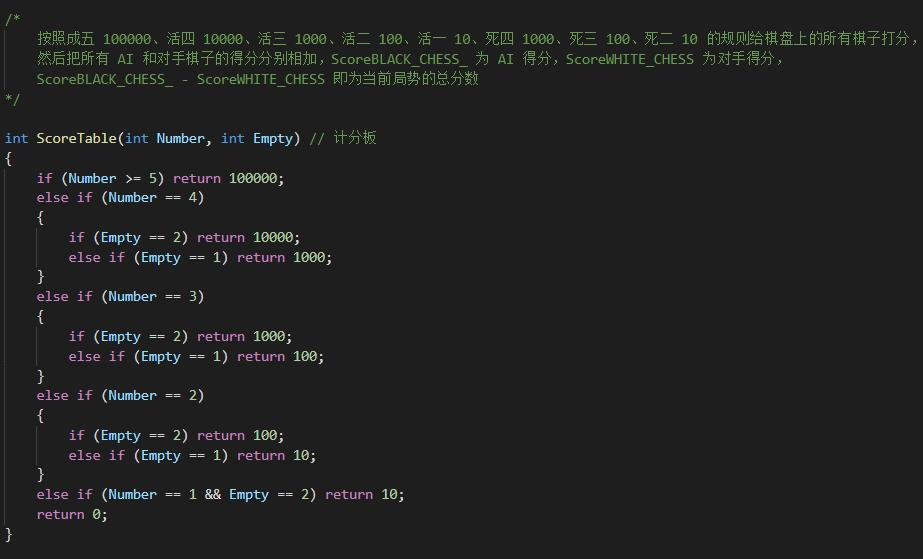
\includegraphics[scale=0.7]{25.jpg}
\caption{26}
\end{figure}
\subsection{统计一行一列或一斜的得分}
\begin{figure}[H]
    \centering
    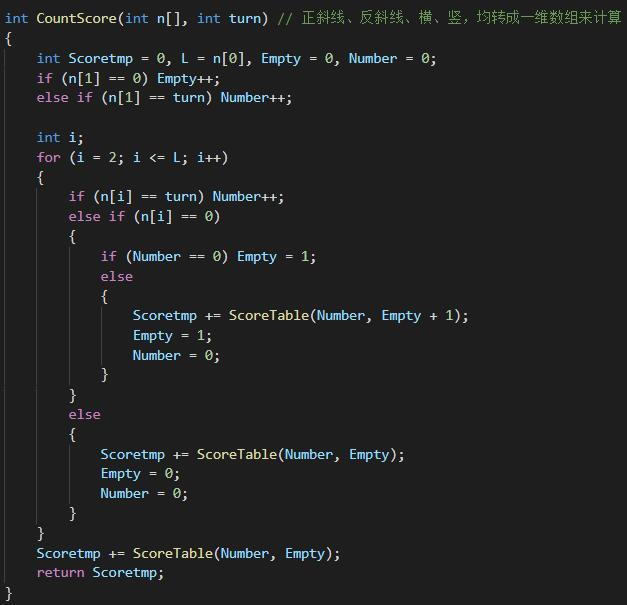
\includegraphics[scale=1.0]{26.jpg}
\caption{27}
\end{figure}
\subsection{评估整个棋局的得分}
\begin{figure}[H]
    \centering
    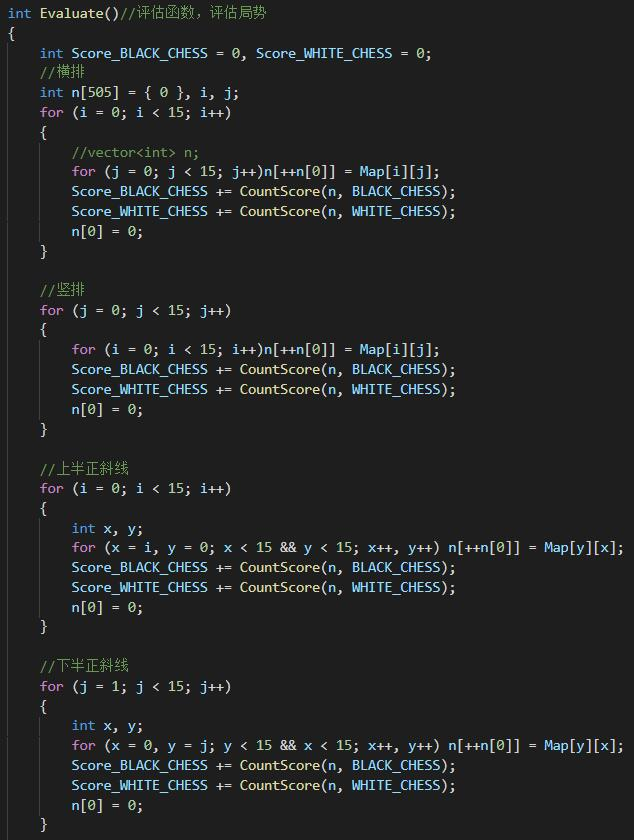
\includegraphics[scale=1.0]{27.jpg}
\caption{28}
\end{figure}
\subsection{最小值搜索(假设人按最优方法下棋)}
\begin{figure}[H]
    \centering
    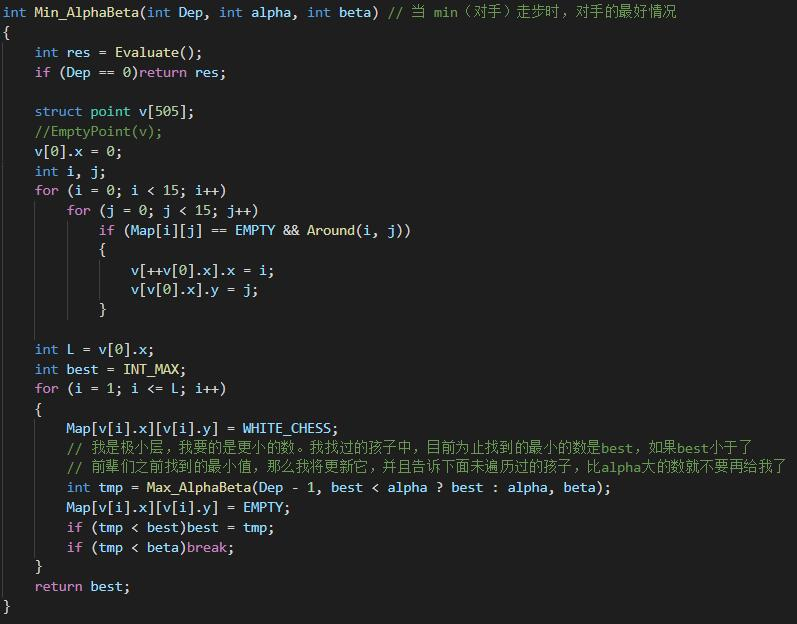
\includegraphics[scale=0.8]{28.jpg}
\caption{29}
\end{figure}
\subsection{最大值搜索(AI用最优的走法)}
\begin{figure}[H]
    \centering
    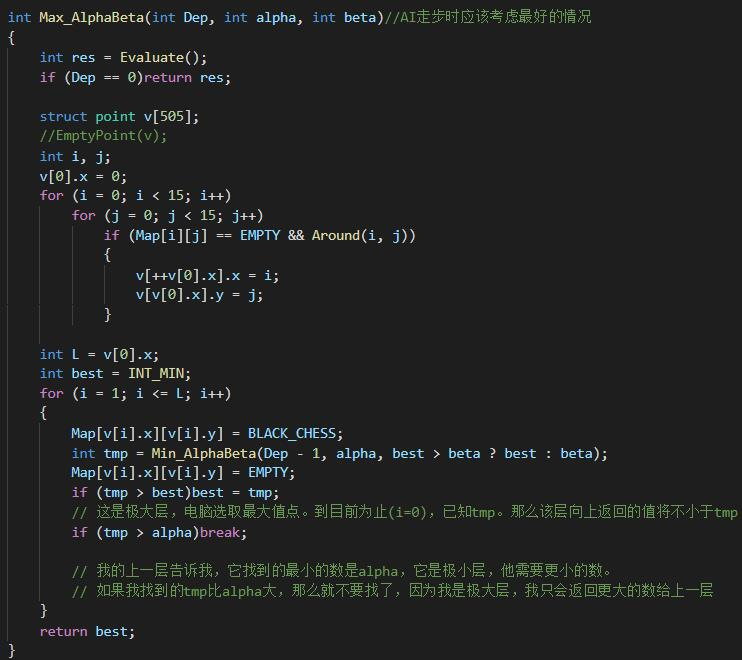
\includegraphics[scale=0.8]{29.jpg}
\caption{30}
\end{figure}
\subsection{alphabeta剪枝算法}
\begin{figure}[H]
    \centering
    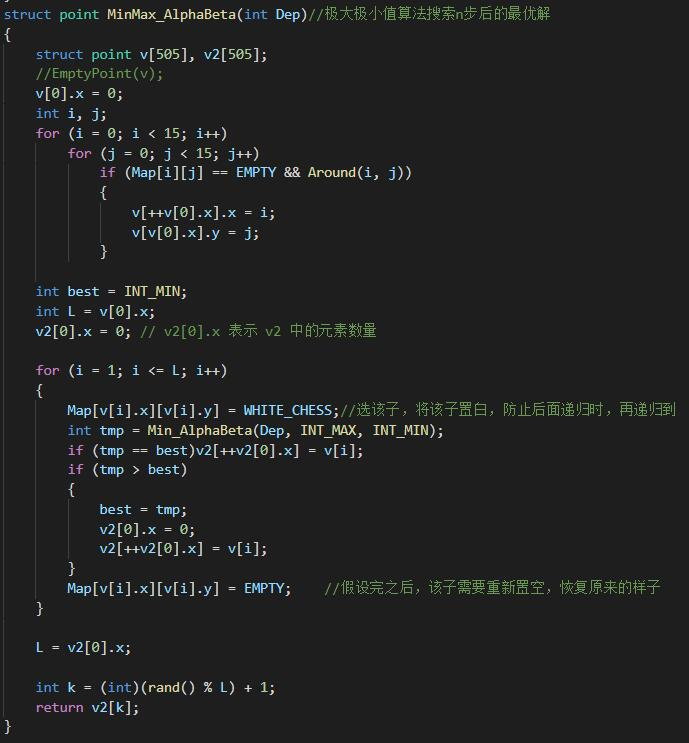
\includegraphics[scale=0.9]{30.jpg}
\caption{31}
\end{figure}
\subsection{返回ai计算出来下棋的点}
\begin{figure}[H]
    \centering
    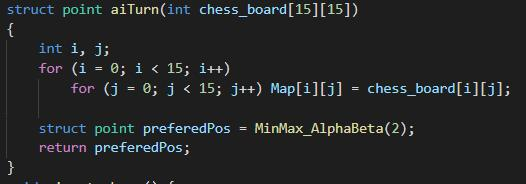
\includegraphics[scale=1.0]{31.jpg}
\caption{32}
\end{figure}
\subsection{ai放置棋子}
\begin{figure}[H]
    \centering
    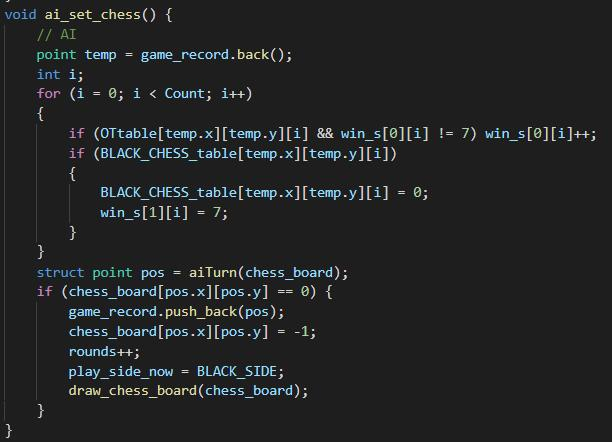
\includegraphics[scale=1.0]{32.jpg}
\caption{33}
\end{figure}
\subsection{检测是否胜利}
\begin{figure}[H]
    \centering
    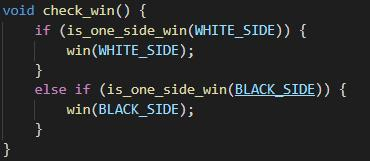
\includegraphics[scale=1.0]{33.jpg}
\caption{34}
\end{figure}
\subsection{展示点赞图片}
\begin{figure}[H]
    \centering
    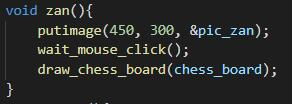
\includegraphics[scale=1.0]{34.jpg}
\caption{35}
\end{figure}
\subsection{展示关于信息}
\begin{figure}[H]
    \centering
    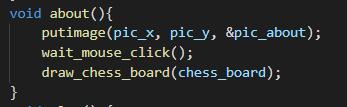
\includegraphics[scale=1.0]{35.jpg}
\caption{36}
\end{figure}
\newpage


\end{document}
